\subsubsection{\stid{2.10} PROTEAS-TUNE - PAPYRUS: Parallel Aggregate Persistent Storage}\label{s:papyrus}

\paragraph{Overview} 
Papyrus is a programming system that provides features for scalable, aggregate, persistent memory in an extreme-scale system for typical HPC usage scenarios. Papyrus provides a portable and scalable programming interface to access and manage parallel data structures on the distributed NVM storage. Papyrus allows the programmers to exploit large aggregate NVM space in the system without handling complex communication, synchronization, replication, and consistency models. Papyrus consists of three components, virtual file system (VFS)~\cite{Kim:2017:DIP}, C++ template container library (TCL)~\cite{Kim:2017:DIP}, and key-value store (KV)~\cite{Kim:2017:PHP}.
%Figure~\ref{fig:papyrus-fig} illustrates the overview of Papyrus.
(1) PapyrusVFS provides a uniform aggregate NVM storage image for the different types of NVM architectures. It presents an illusion of a single large NVM storage for all NVM devices available in the distributed system. Unlike other traditional kernel-level VFSs, PapyrusVFS is a lightweight user-level VFS, which is provided as a library so that applications can link to or dynamically load it. PapyrusVFS implements a subset of POSIX API related to file I/O. (2) PapyrusTCL provides a high-level container programming interface whose data elements can be distributed to multiple NVM nodes. PapyrusTCL provides three containers, including map, vector, and matrix, implemented as C++ templates. PapyrusTCL is built on top of PapyrusVFS. This enables PapyrusTCL to be decoupled from a specific NVM architecture and to present a high-level programming interface whose data elements are distributed across multiple NVM nodes transparently. (3) PapyrusKV is a novel embedded KVS implemented specifically for HPC architectures and applications to provide scalability, replication, consistency, and high performance, and so that they can be customized by the application. It stores keys and values in arbitrary byte arrays across multiple NVMs. PapyrusKV provides configurable consistency technique controlled by the application during the program execution dynamically to meet application-specific requirements and/or needs. It also supports fault tolerance and streamlined workflow by leveraging NVM's persistence property.

%\begin{figure}[htb]
%    \centering
%    \includegraphics[width=5in]{papyrus-fig}
%    \caption{\label{fig:papyrus-fig}Papyrus consists of three components, virtual file system, C++ template containers, and key-value store}
%\end{figure}

\paragraph{Key Challenges}
In HPC, NVM is quickly becoming a necessary component of future systems, driven, in part, by the projections of very limited DRAM main memory per node and plateauing I/O bandwidth. More concretely, recently-announced DOE systems, such as NERSC's Cori, LANL/Sandia's Trinity, LLNL's Sierra, OLCF's Summit, TACC's Stampede2, and ALCF's Theta, include some form of NVM. This NVM will be used in two fundamental ways. First, it will be used as a cache for I/O to and from the traditional HDD-based external parallel file systems. In this case, most scientists believe that the caching can be implemented transparently, shielding complexity from the applications and users. Second, NVM will be used as an extended memory to provide applications with access to vast amounts of memory capacity beyond what is feasible with DRAM main memory. More interestingly, in HPC, this extended memory can be aggregated into a much larger, scalable memory space than that provided by a single node alone. In this second case, however, no portable and scalable programming systems exist.

\paragraph{Solution Strategy}
We describe our key goals for Papyrus: high performance, scalability, portability, interoperability with existing programming models, and application customizability. First, \textbf{high performance} is a clear need in HPC. The design of Papyrus should provide the opportunity to exploit NVM resources efficiently. Second, \textbf{scalability} is important in HPC as most of the applications must run on large sectors of the systems - thousands to hundreds of thousands of processors. Papyrus should not inhibit scalability; it should provide an interface that is able to scale as the application and system do. Third, \textbf{portability} is a necessary requirement because HPC applications must be able to run on multiple, diverse platforms at any given time. The upcoming DOE systems all have NVM integrated into the systems in different ways. Papyrus must provide both functional portability and performance portability across systems with different architectures. Fourth, \textbf{interoperability} is a practical requirement of HPC applications. Papyrus must be designed so that it can be incrementally introduced into an application without conflicting with existing HPC programming models and languages like MPI, UPC, OpenMP, OpenACC, C, C++, and Fortran. Furthermore, Papyrus should leverage characteristics of these other programming models when possible. Interoperability allows programmers to adopt Papyrus incrementally in legacy MPI applications avoiding major rewrites of the application. Fifth, \textbf{application customizability} is a key requirement to achieve high performance and scalability. HPC applications have many different usage scenarios, and thus Papyrus should have customizable parameters for key features that impact other important properties like performance and scalability.

\paragraph{Recent Progress}

Meraculous~\cite{Georganas:2014:PDB} is a state-of-the-art de novo assembler written in UPC. Its parallel algorithm for de Bruijn graph construction and traversal leverages the one-sided communication in UPC to facilitate the requisite random access pattern in the global de Bruijn graph. The de Bruijn graph is implemented as a distributed hash table with an overlapping substring of length {\it k}, referred to as a {\it k-mer}, as key and a two-letter code [ACGT][ACGT] as value as shown in \autoref{fig:papyrus-meraculous}. A hash function is used to define the affinities between UPC threads and hash table entries. We ported the distributed hash table written in UPC to a PapyrusKV database. The keys in the database are k-mers and the values are two-letter codes. The PapyrusKV runtime calls the same hash function in the UPC application to determine the owners of key-value pairs in the database by specifying the custom hash function when the database is created. Thus, the thread-data affinities in UPC and PapyrusKV are the same as shown in \autoref{fig:papyrus-meraculous}. PapyrusKV requires fewer lines of source code than UPC because it calls standard put and get API functions without implementing an application-specific algorithm for the distributed hash table construction and traversal. \autoref{fig:papyrus-meraculous-eval} shows the performance comparison between PapyrusKV and UPC of Meraculous on Cori. Both versions are built and run using Berkeley UPC, an MPI-interoperable UPC implementation. We measured the total execution time on 32, 64, 128, 256, and 512 UPC threads (32 UPC threads per node). UPC shows better performance than PapyrusKV due to its RDMA capability and built-in remote atomic operations during the graph traversal. The performance gap between UPC and PapyrusKV decreases as the number of UPC threads increases. On 512 UPC threads, PapyrusKV runs 1.5 times slower than UPC. This is mainly because of the asynchronous migration in PapyrusKV during the graph construction.

%\begin{figure}[htb]
%\centering
%\includegraphics[width=3in]{projects/2.3.2-Tools/2.3.2.09-PROTEAS/papyrus-meraculous}
%\caption{K-mer distributed hash table implementations in UPC and PapyrusKV.}
%\label{fig:papyrus-meraculous}
%\end{figure}
%
%\begin{figure}[htb]
%\centering
%\includegraphics[width=3in]{projects/2.3.2-Tools/2.3.2.09-PROTEAS/papyrus-meraculous-eval}
%\caption{Meraculous performance comparison between PapyrusKV (PKV) and UPC on Cori.}
%\label{fig:papyrus-meraculous-eval}
%\end{figure}


\begin{figure}[t]
    \centering
    \begin{subfloat}[K-mer distributed hash table implementations in UPC and PapyrusKV.\label{fig:papyrus-meraculous}]
        \centering
        \includegraphics[width=.48\textwidth]{projects/2.3.2-Tools/2.3.2.10-PROTEAS-YTUNE/papyrus-meraculous}
    \end{subfloat}
    \hfill
    \begin{subfloat}[Meraculous performance comparison between PapyrusKV (PKV) and UPC on Cori.\label{fig:papyrus-meraculous-eval}]
        \centering
        \includegraphics[width=.48\textwidth]{projects/2.3.2-Tools/2.3.2.10-PROTEAS-YTUNE/papyrus-meraculous-eval}
    \end{subfloat}
    \caption{Using PapyrusKV for Meraculous.}
\end{figure}

%\begin{figure}[t]
%    \centering
%    \begin{subfigure}[b]{0.45\textwidth}
%        \includegraphics[width=.99\textwidth]{projects/2.3.2-Tools/2.3.2.09-PROTEAS/papyrus-meraculous}
%        \caption{K-mer distributed hash table implementations in UPC and PapyrusKV.}
%        \label{fig:papyrus-meraculous}        
%    \end{subfigure}
%    \hfill
%    \begin{subfigure}[b]{0.45\textwidth}
%        \includegraphics[width=.99\textwidth]{projects/2.3.2-Tools/2.3.2.09-PROTEAS/papyrus-meraculous-eval}
%        \caption{Meraculous performance comparison between PapyrusKV (PKV) and UPC on Cori.}
%        \label{fig:papyrus-meraculous-eval}
%    \end{subfigure}
%    \caption{Using PapyrusKV for Meraculous.}
%\end{figure}


This past year, we have added data compression and encryption to Papyrus. For data compression, the overhead of data access and movement becomes a serious bottleneck compared to compute overhead in large-scale HPC systems. We integrated data compression methods into Papyrus to achieve storage reduction and performance improvement. 
For data encryption, we need to protect sensitive data (e.g., health records, DNA data) that is being used in distributed infrastructures, and users need practical methods to secure their data throughout its lifecycle. We will introduce data encryption in Papyrus to add an extra layer of security in the complex scientific workflows.


\paragraph{Next Steps}
Our next efforts are:

\begin{enumerate}
\item \textbf{Versioning: } Versioning can be used to provide new levels of reliability and performance optimization. We will design and implement versioning in Papyrus.

\item \textbf{Performance optimization:} New APIs and hardware support is being developed for NVM technologies; we are implementing optimizations in Papyrus to take advantage of these advances.

\end{enumerate}
